\section{Layered Grid Architecture}\label{layered_grid_architecture}
Following the work of Ian Foster, Carl Kesselman and Stevel Tuecke \cite{the_anatomy_of_the_grid}, the Grid Architecture identifies fundamental system components, and indicates how these components interact with one another. This \textbf{Grid Architecture is first and foremost a protocol architecture}, since the \textbf{interoperability among any potential participant is the central issue} and thus requires the definition of common protocols. Protocols govern the \textit{interaction} among components in the Grid and not the \textit{implementation}, maintaining local control.

\begin{quotation}
    \textit{"Why are protocols critical to interoperability? A protocol definition specifies how distributed system elements interact with one another to achieve a specified behavior and the structure of the information exchanged during this interaction. This focus on externals (interactions) rather than internals (software, resource characteristics) has important pragmatic benefits." \cite{the_anatomy_of_the_grid}}
\end{quotation}

In order to provide abstractions to interact with the Grid and develop applications that use it, application programming interfaces (\textbf{APIs}) and software development kits (\textbf{SDKs}) must also be provided; these are built on top of the protocols.
Together, APIs, SDKs and the protocols in the architecture constitute a \textbf{middleware}.

The architecture is organized in a \textbf{layer structure} (\textit{figure \ref{fig:grid_protocol_architecture_and_internet_protocol_architecture}}), where components within each layer share common characteristics but can build on capabilities and behaviors provided by any lower level. \textbf{The number of protocols must be contained}, focusing on Resource and Connectivity protocols.

\begin{figure}[!ht]
    \centering
    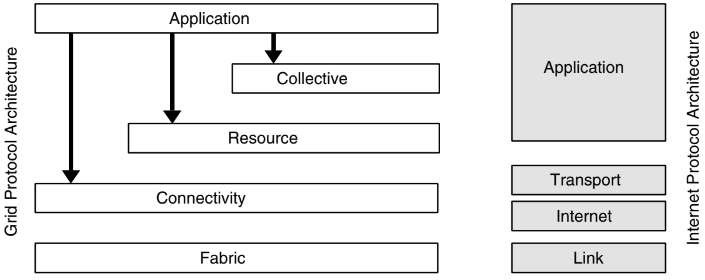
\includegraphics[scale=1]{document/chapters/chapter_2/images/grid_protocol_architecture_and_internet_protocol_architecture.png}
    \caption{Layered architecture relationship to Internet Protocol (IP) architecture. \cite{the_anatomy_of_the_grid}}
    \label{fig:grid_protocol_architecture_and_internet_protocol_architecture}
\end{figure}

\subsection{Fabric layer}
\begin{figure}[!ht]
    \centering
    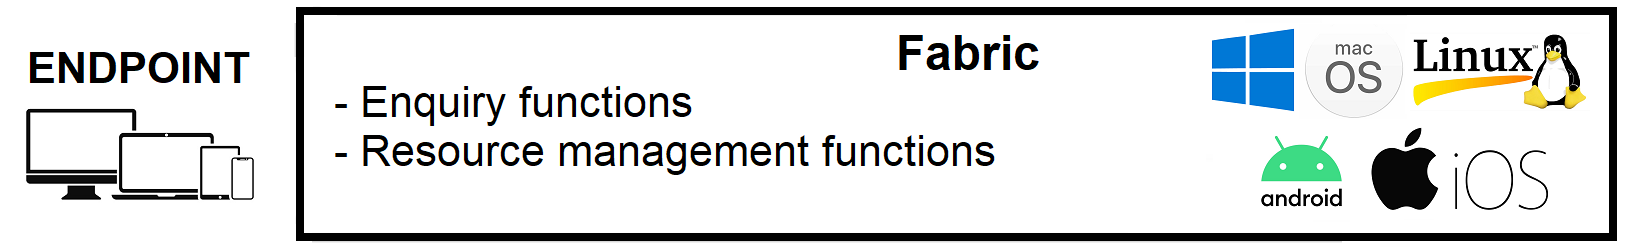
\includegraphics[scale=0.35]{document/chapters/chapter_2/images/fabric_layer.png}
    \caption{Layered Grid Architecture - Fabric layer}
    \label{fig:fabric_layer}
\end{figure}

\noindent This is the layer that \textbf{implements the local, resource-specific operations that occur on specific resources} (whether physical or logical) \textbf{as a result of sharing operations at higher levels}. The external access to such resources is mediated by protocols defined in the Grid, while \textbf{the internal workings of this layer depend on the specific implementation that runs on a machine}; this organization results in a relatively tight interdependence between the operations defined in this layer and the operations defined in higher layers.
\vspace{30mm}

\textbf{Operations in this layer should be as simple and minimal as possible in order to easily extend compatibility with as many devices as possible}; said operations must involve:
\begin{itemize}
    \item \textbf{Enquiry functions}\\
    Allow to discover the Node inside the Grid, as well as describe its resources and status. Resources description provides info about software and hardware capabilities, while status handling offers mechanisms to enquire current load and queue state.
    \item \textbf{Resource management mechanisms}\\
    Allow performing operations using the resources offered by the Node, such as access to storage, computation and network.
\end{itemize} 
\vspace{5mm}

\subsection{Connectivity layer}\label{connectivity_layer}
\begin{figure}[!ht]
    \centering
    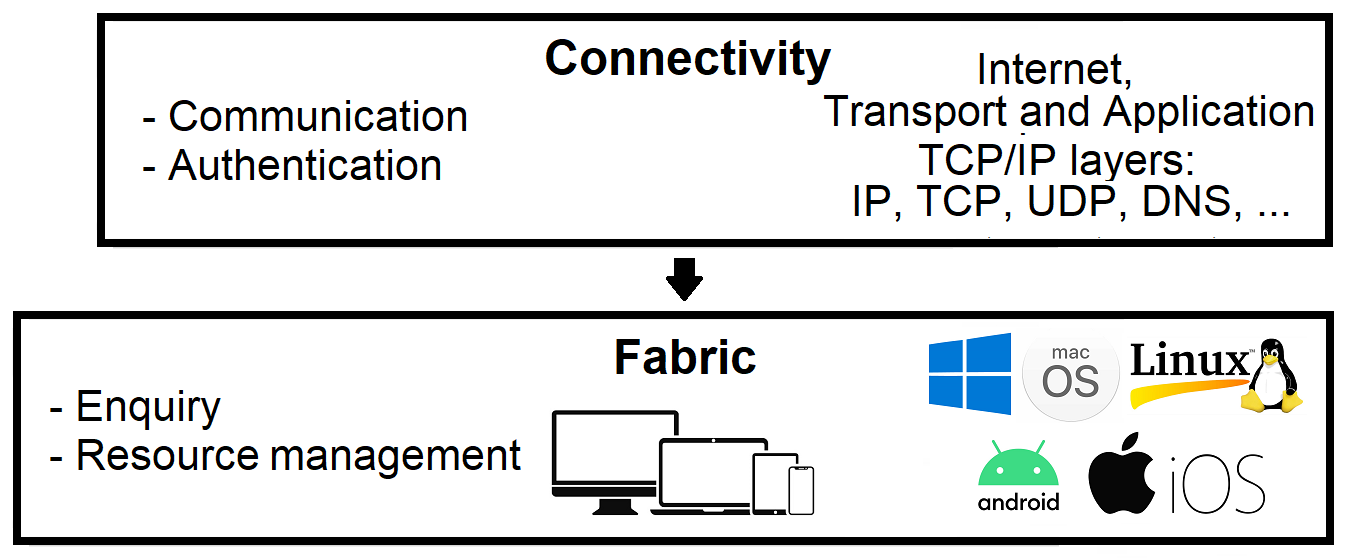
\includegraphics[scale=0.35]{document/chapters/chapter_2/images/connectivity_layer.png}
    \caption{Layered Grid Architecture - Connectivity layer}
    \label{fig:connectivity_layer}
\end{figure}
\vspace{5mm}

\noindent This layer \textbf{defines core communication and authentication protocols that are used for network transactions inside the Grid} in order to enable the exchange of data among fabric layer resources.
\begin{itemize}
    \item \textbf{Communication protocols}\\
    This protocols handle transport, routing and naming. Here, technologies are mapped to the TCP/IP stack, in particular to the Internet, Transport and Application layers; communication is built on already well-established protocols like IP, TCP, UDP, DNS, etc... 
    \item \textbf{Authentication protocols}\\
    Mechanisms regarding authentication must possess the following characteristics:
    \begin{itemize}
        \item \textit{Single sign-on}: users authenticate just once, and then they have access to a multitude of resources;
        \item \textit{Delegation}: a user should allow executing authorized instructions on their machine; 
        \item \textit{Integration with various local security solutions}: the layer should include security solutions provided by the local machine;
        \item \textit{Enable users' control over authorization}: the user must be able to change authorizations regarding the resources that their machine offers.
    \end{itemize}
\end{itemize}

\subsection{Resource layer}\label{resource_layer}
\begin{figure}[!ht]
    \centering
    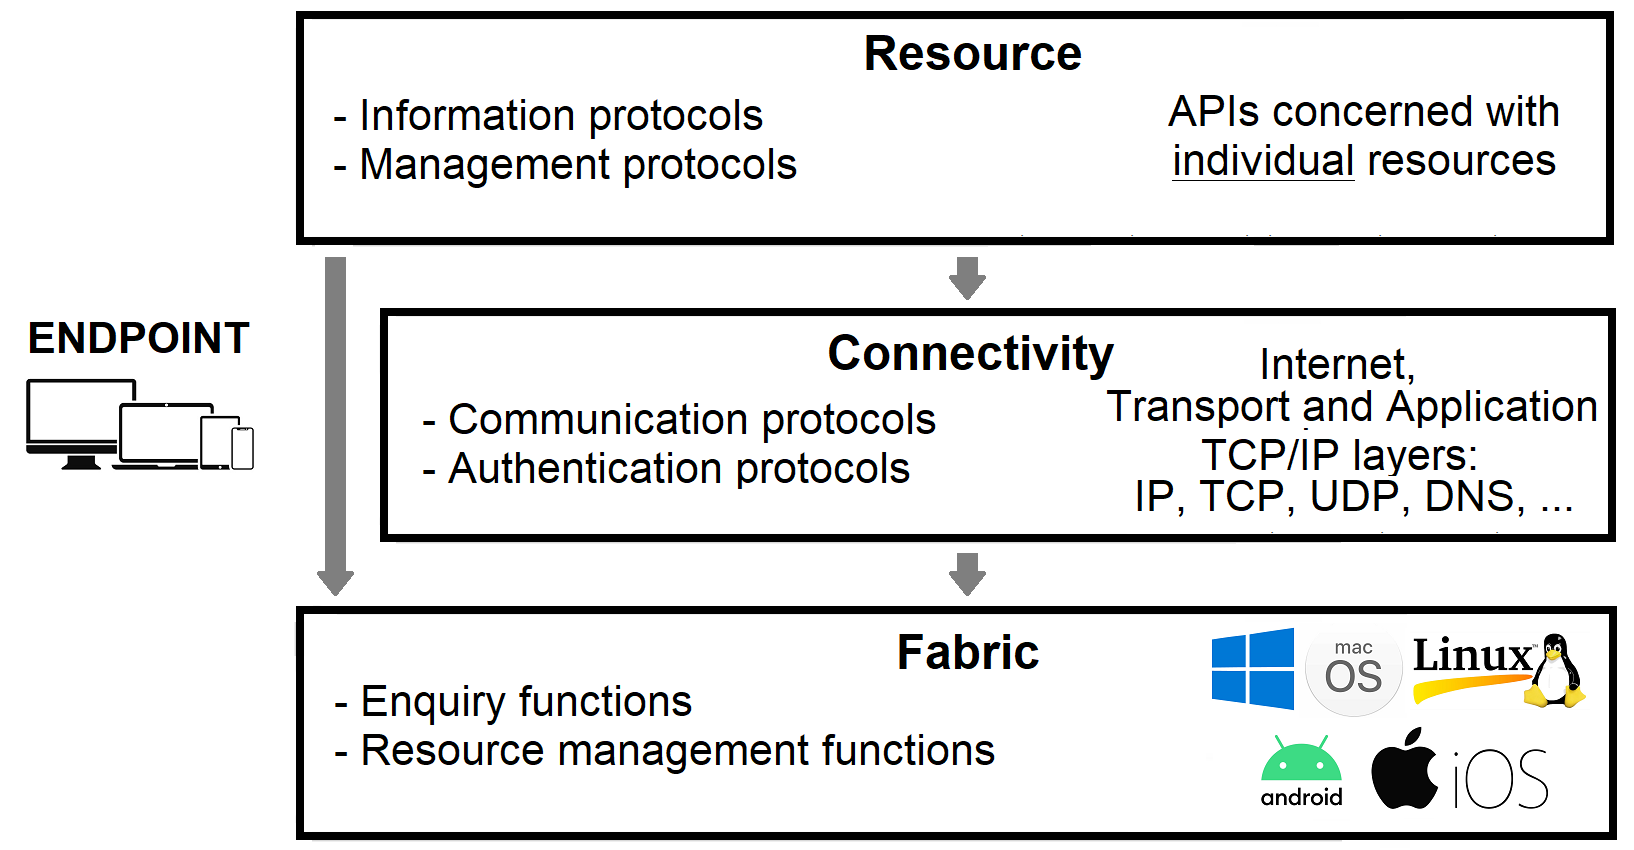
\includegraphics[scale=0.35]{document/chapters/chapter_2/images/resource_layer.png}
    \caption{Layered Grid Architecture - Resource layer}
    \label{fig:resource_layer}
\end{figure}

\noindent In the Resource layer, the primary focus is \textbf{the secure negotiation, initiation, monitoring, control, accounting and payment of \textit{individual} resources}; this means that \textbf{this layer is not concerned with the global state the Grid is in} (that will be handled in the Collective layer), but it just deals with communicating with a single machine. Here, protocols should be limited to a small set that captures fundamental mechanisms of sharing across different resource types while, at the same time, not overly constraining higher protocols defined in the Collective and Application layers.

Implementations of the Resource layer \textbf{rely upon functions defined at fabric layer in combination with previous layer's communication and authentication protocols}, resulting in creating \textbf{APIs} used to utilize this layer's capabilities.
Two protocol classes are defined at this level:
\begin{itemize}
    \item \textbf{Information protocols}\\
    Provide information about the structure and state of a resource (ex: configuration, current load, usage policy, etc...).
    \item \textbf{Management protocols}\\
    Deal with the negotiation process performed in order to access a shared resource (resource requirements, operations to be performed and applying usage policies).
\end{itemize} 

\subsection{Collective layer}
\begin{figure}[!ht]
    \centering
    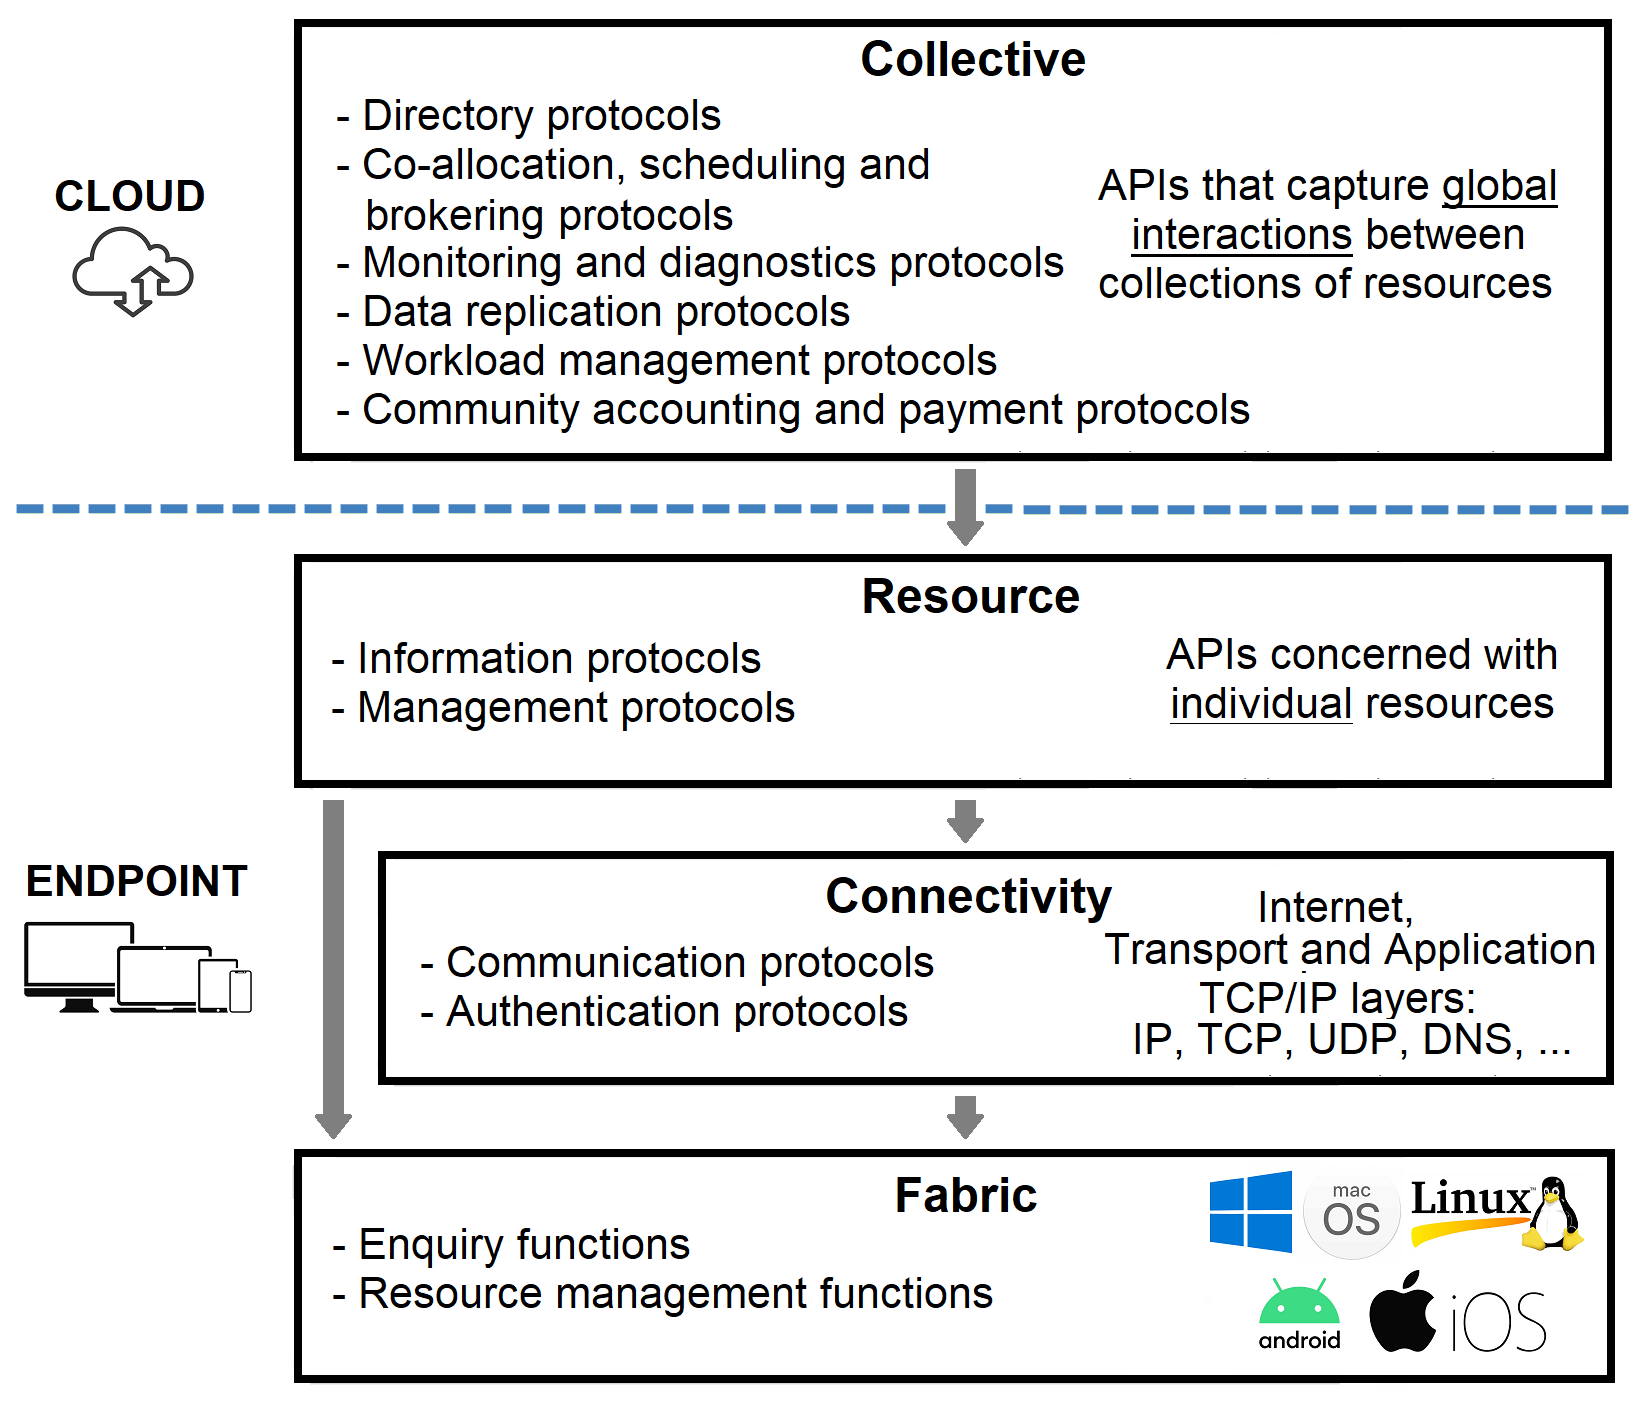
\includegraphics[scale=0.34]{document/chapters/chapter_2/images/collective_layer.png}
    \caption{Layered Grid Architecture - Collective layer}
    \label{fig:collective_layer}
\end{figure}

\noindent Here the main focus shifts from the management of a single specific resource to \textbf{dealing with questions that are global in nature, capturing interactions across collections of resources}. Previous layers dominated the realm of a single machine (with its resources) acting as an endpoint, but this layer changes context, becoming a \textbf{cloud-based domain}.

If the limited number of protocols at the Resource layer are well-designed, \textbf{this layer can offer a wide variety of sharing behaviors} that build upon those protocols. Such sharing behaviors depend on what capabilities the Grid wants to offer. Those behaviors, that are then accessed by using APIs, \textit{can} include:
\begin{itemize}
    \item \textbf{Directory protocols}\\
    Used to discover and query resources by name and/or attributes such as availability, type and workload.
    \item \textbf{Co-allocation, scheduling and brokering protocols}\\
    With such protocols, resources are assigned and allocated for a specific purpose in order to execute a scheduled task.
    \item \textbf{Monitoring and diagnostics protocols}\\
    Through these protocols resources are monitored for failure, overload, external attacks, etc...
    \item \textbf{Data replication protocols}\\
    In order to maximize performances, these protocols manage data replication to increase reliability while reducing response time.
    \item \textbf{Workload management protocols}\\
    Used to solve situations where, through information obtained using discovery protocols, an excessive workload is detected.
    \item \textbf{Community accounting and payment protocols}\\
    Such protocols collect information about Grid usage; with such information payments involving resources usage can occur.
    \item \textbf{Grid-enabled programming systems protocols}\\
    Lastly, these protocols offer familiar grid-enabled programming models and paradigms to be used to perform computations inside the Grid. 
\end{itemize}

\subsection{Application layer}
\begin{figure}[!ht]
    \centering
    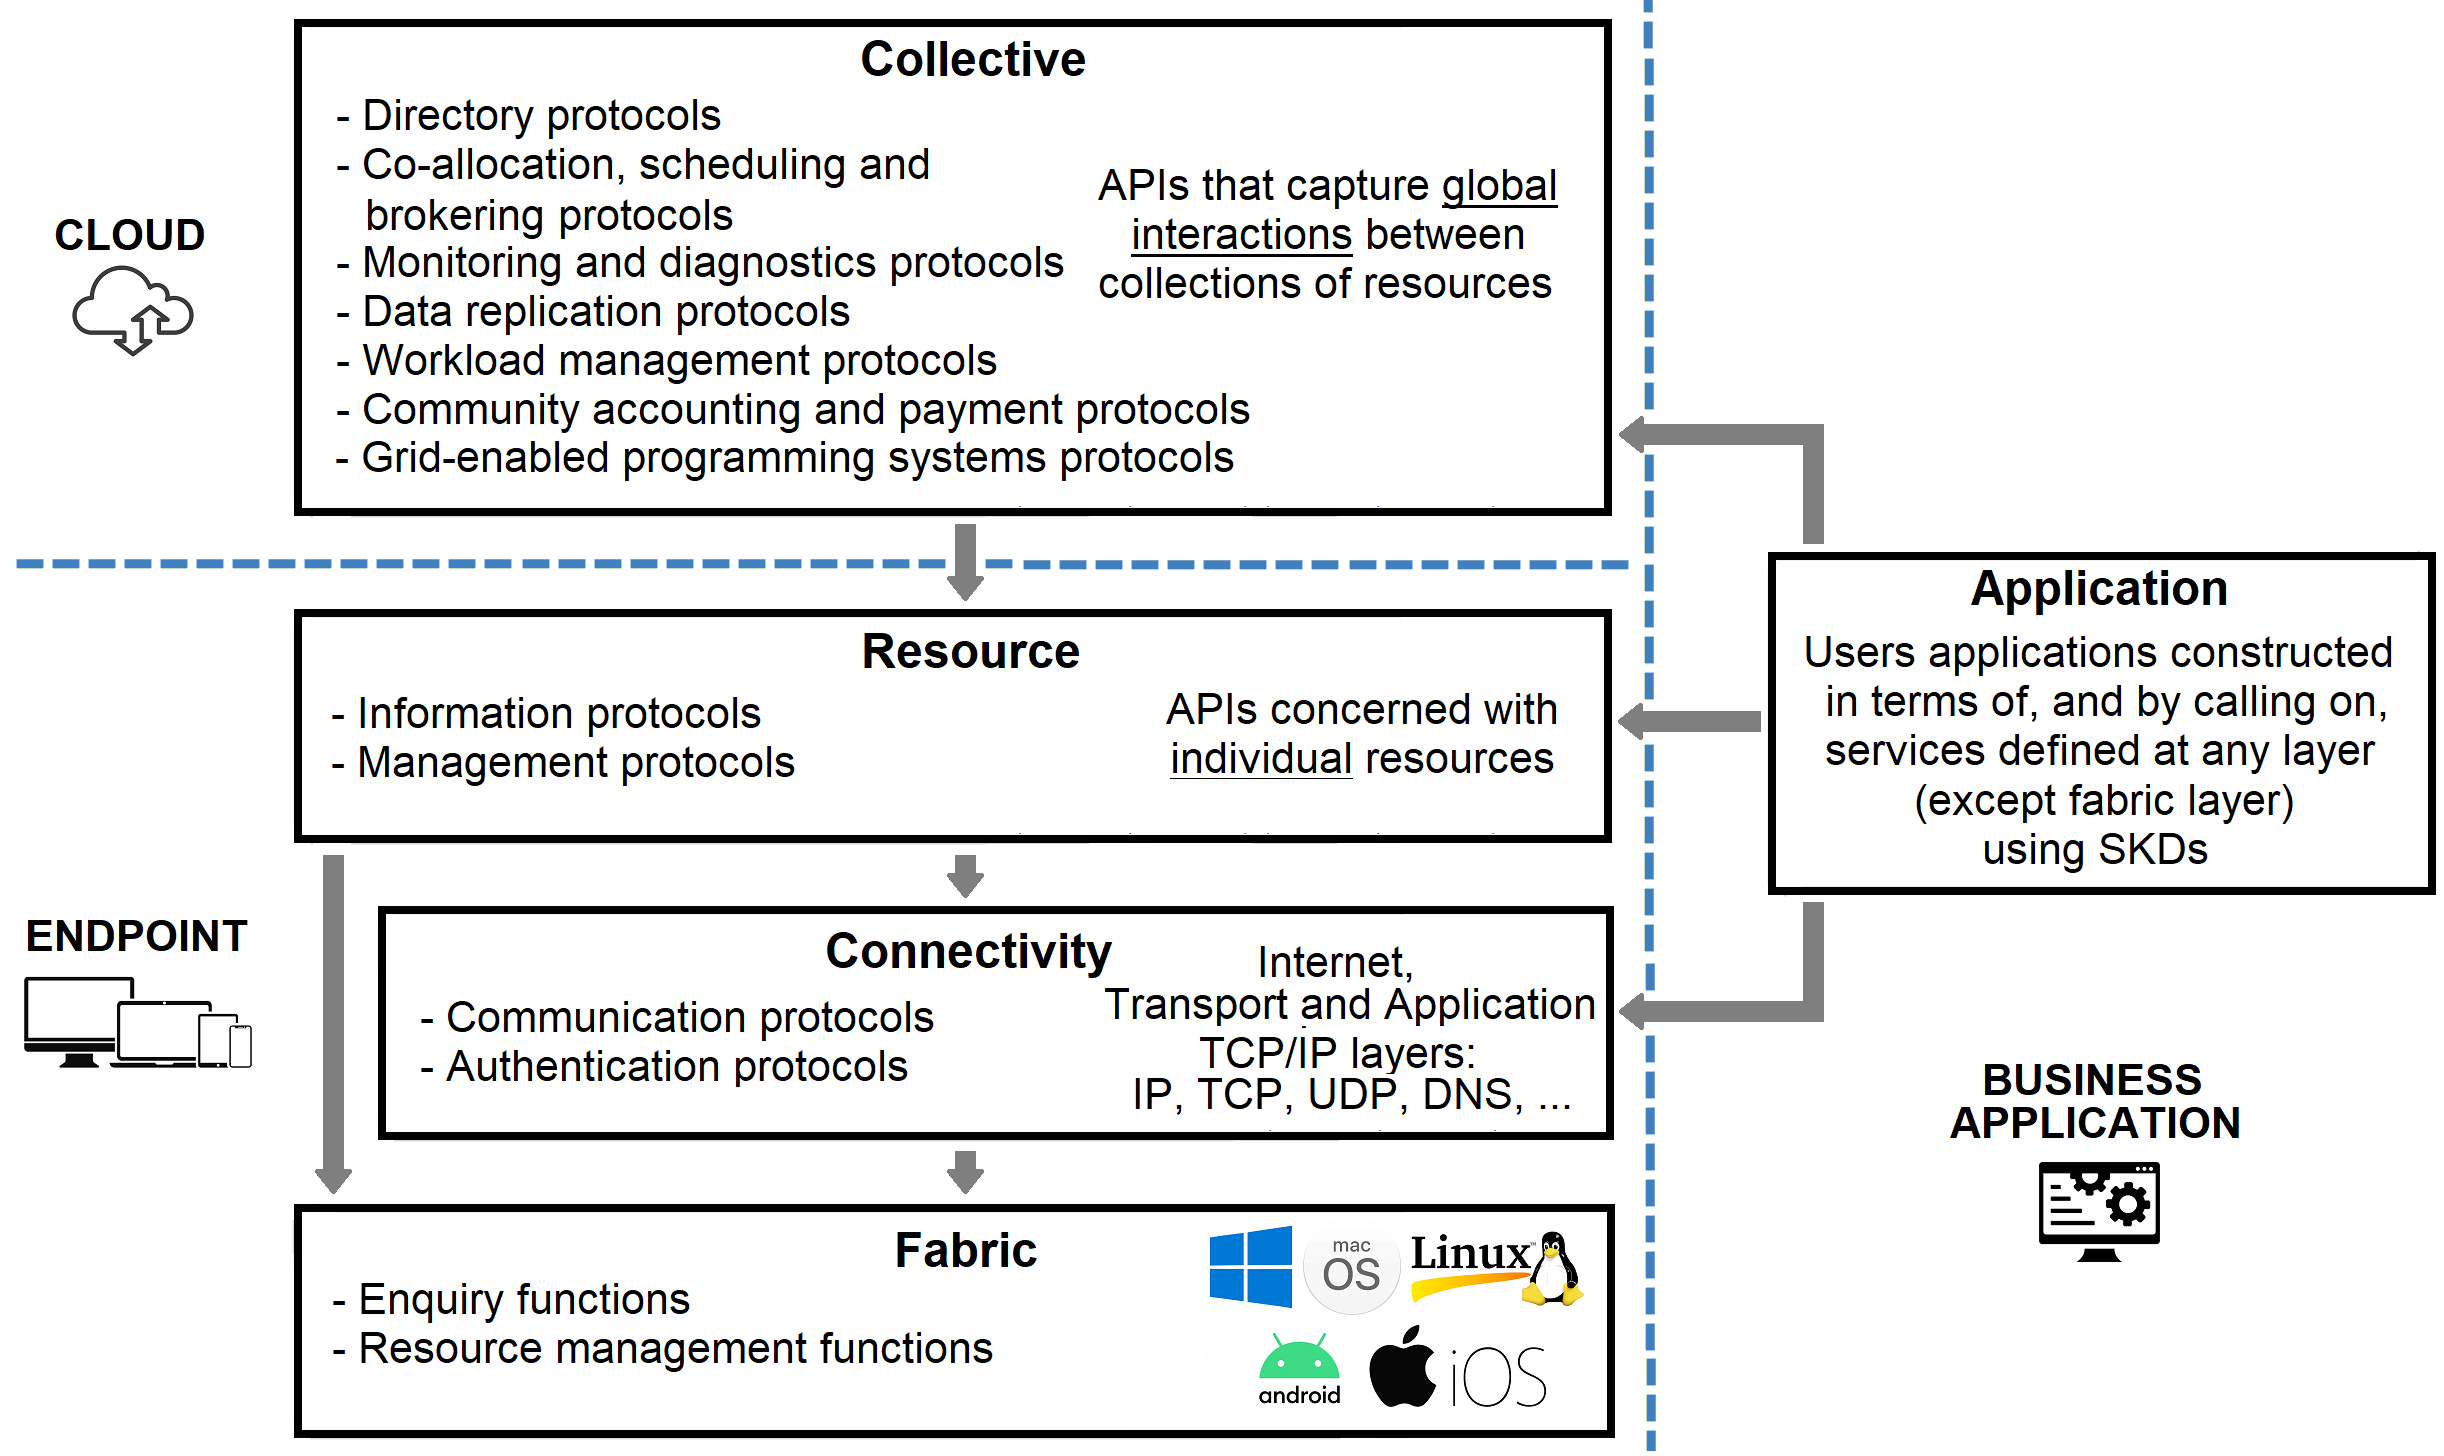
\includegraphics[width=\linewidth]{document/chapters/chapter_2/images/application_layer.png}
    \caption{Layered Grid Architecture - Application layer}
    \label{fig:application_layer}
\end{figure}

\noindent The final layer constitutes \textbf{all the applications that use services offered by the Grid}; the \textbf{desired behavior for the user application is constructed in terms of, and by calling on, services defined at any layer} (except fabric layer), accessed via an SDK provided by the implementor of the Grid; through a combination of services defined in the other layers, software development and, possibly, collaborating with third party libraries, more complex behaviors can be built in order to satisfy specific use cases.
